	The questionnaire's flow captures the sequence for the question constructs defined in a questionnaire. The designers or social researchers commonly use skip patterns that can be interchanged with filters to express the logical order of elements in a questionnaire. We have explored the directed graphs, Petri Nets and the hierarchical paradigms in order to %find out whether these approaches describe questionnaires in a structured manner but permitting designers to express logics through skip patterns.
	establish the suitability for representing sequence logic.

	The \emph{directed graph}, was explored in the past by Fagan et al. in order to analyse the use of skip constructs on surveys. These graphs based on \emph{nodes} and \emph{arcs} are able to represent question and response choices respectively. %Moreover, the source and sink properties of the graph correspond to the first and last question of a questionnaire. 
	When additional information such as the conditions that determine the ordering of questions are added to these graphs, they become flowcharts which result in tools to document and understand questionnaire's flow \cite{art:jabine85}. The directed graphs, permit validating the correctness of data gathered from surveys by detecting whether or not a question response is missed or is not applicable. These verifications are conducted applying different graph properties \cite{tech:fagan88}. Although the properties from graphs can be used to model the flow of questionnaires, as far as we know, this paradigm has not been used to formally define questionnaire specifications in \gls{xml}.

	In more recent work, Petri Nets have been applied to visualise and analyse complex questionnaires \cite{proc:rolke10}. Figure \ref{fig:literature:pretiNet} illustrates the Petri Net representation on part of the questionnaire from Figure \ref{fig:background:survey} in relation to question Q1 and the skip construct that permit navigating either to Q2 or END. %A more recent study case carried out by Rolke is concentrated on the visualisation and analysis of a complex questionnaire using Preti Nets. Figure \ref{fig:literature:pretiNet} contains a small portion of this net that represents part of the paper questionnaire from Figure \ref{fig:background:survey}. Specifically, it is depicted the question Q1 and the skip construct that permit navigating either to Q2 or END. 
	Here a \emph{place} (e.g. Q1, Q2 and END) captures the static information from a question whereas a transition (e.g. 01, 02, 03, 04, 05) represents a response choice. Additionally exist \emph{arcs} to connect places to transitions (e.g. arrow connecting Q1 to 01) and vice versa (e.g. 01, 02 and 03 to END). A Petri Net permits validating the \emph{reachability} of places, i.e. checking whether or not a set of responses given for questions correspond to a valid state of the net. However, this modelling approach is only limited to finite domain, i.e. it is only applicable for single and multiple questions, but becomes hard to manage open questions since an arc connecting places to/from transitions has to be specified for any possible value expected.

	\begin{figure}[h]
	\centering
	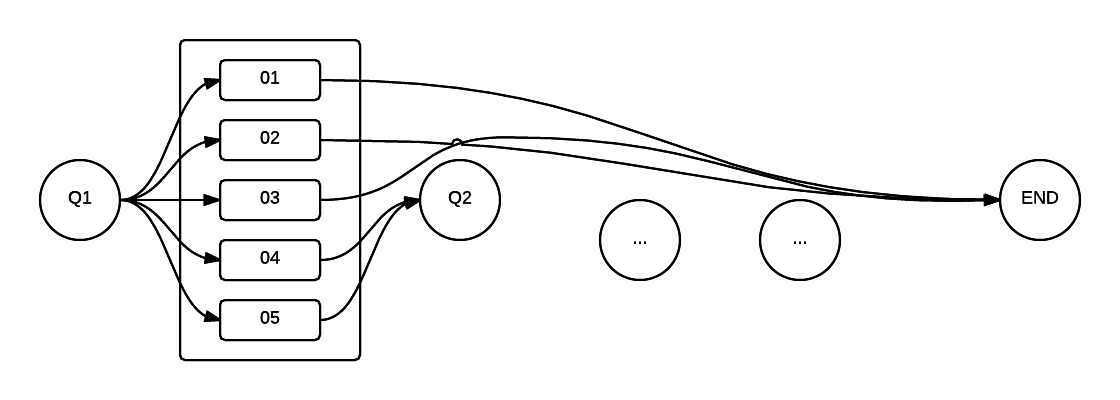
\includegraphics[max size={\textwidth}{\textheight}]{literature/img/pretiNet.png}
	\caption{Petri Net instance}
	\label{fig:literature:pretiNet}
	\end{figure}

	\gls{sss}, \gls{ddi} and \gls{qdl} adopt a hierarchical modelling approach where the use of skip pattern is avoided in favour of structured constructs (if-then-else, loops and sequences) as advocated by Dijkstra \cite{art:dijkstra68}. As such, the routing structure of surveys can be seen as trees permitting not only the identification of the path followed but also determining all the circumstances under which a question may be triggered \cite{web:spencer12}. Algorithm \ref{alg:hierarchical} describes in pseudo-code the routing of the questionnaire from Figure \ref{fig:background:survey} according to the hierarchical modelling. Note how the nesting of constructs is used to avoid skips. However, this nesting is not naturally well suited to reusability.%WEIRD does not naturally well suited ...

	\begin{algorithm}
	INF1\;
	Q1\;
	\If{NOT(Q1 IS\_SEL '01' OR Q1 IS\_SEL '02' OR Q1 IS\_SEL '03')}{
		Q2\;
		\If{NOT(Q2 IS\_SEL '99')}{
			Q3\;
			\If{NOT(Q3 IS\_SEL '99')}{
				Q4\;
				\If{Q2 IS\_SEL '06'}{
					Q5\;
					\For{each Q2 SEL}{
						Q6a\;
					}
					\If{HAD\_CAR \textgreater 1}{
						INF2\;
					}
				}
			}
		}
	}
	END\;
	\caption{Hierarchical modelling example}
	\label{alg:hierarchical}
	\end{algorithm}

	The benefits of eliminating skip patterns are universally acknowledged by high-level programme languages architects, however designers or social researchers still specify questionnaires through documents using skips to navigate from one question to another \cite{proc:katz97}, not only because they do not have programming skills but also because the final client interested in the survey, demands plain English instructions. As the hierarchical approach replaces the use of skip constructs, there is an evident \emph{gap} between what the social researchers design versus the \emph{code} that a \gls{cawi} system uses to execute a survey. Costigan states that having two sources of specification, i.e. the code and the document requires duplication of effort and it is prone to error \cite{proc:costigan03}. To unify these two sources, Spencer proposes that researchers should be trained to use structured patterns \cite{web:spencer12}, i.e. avoid the use of skip constructs. However, in practice, motivating social researchers to adopt this practice remains a problem \cite{proc:costigan03}. %few social researchers would be interesting in eliminating skip patterns from questionnaire specifications \cite{proc:costigan03}.

	The ability to introduce changes to questionnaires is another factor to consider since clients often demand the modification of survey logics when the data collection is already taking place. This involves having a modelling approach that addresses the \emph{adaptability} appropriately. It is evident from the above hierarchical representation that strong coupling between the inner and outer filters increases with increasing skip constructs. %It is evident by examining the above example introduced, that exist coupling between the inner and outer filters which increases when newer skip constructs are added. 
	As dependencies among constructs are like to impact negatively to changes to questionnaire's flow, there is a need to explore a less intrusive model.
	